% Utiliser des sections et des subsections pour les différentes parties du document.
% Utiliser begin{figure} pour les images sans oublier les labels pour le référencement

\section{Présentation générale}

\subsection{Archétype}

Notre but est de réaliser un jeu stratégique au tour par tour semblable à Advance Wars


\begin{figure}[h]
    \centering
    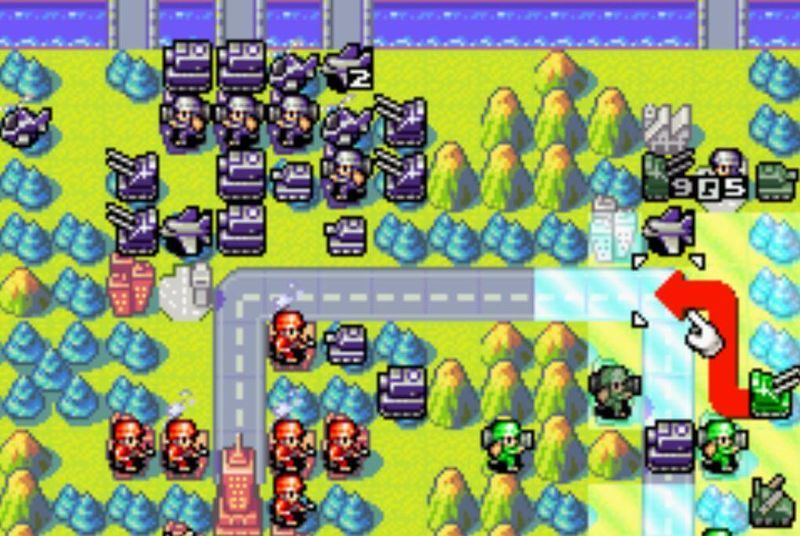
\includegraphics[scale = 0.5]{images/advanceWarsGameplay.jpg}
    \caption{Sprite des tuiles}
    \label{fig:Advance Wars}
\end{figure}


\subsection{Règles du jeu}

Notre jeu, "Until The Last Barrel", est un jeu de stratégie au tour par tour dont le but est de vaincre ses adversaires en capturant son Quartier Général (QG) sur le champ de bataille. Le dernier joueur survivant est donc déclaré vainqueur.
Pour se faire le joueur dispose de trois ressources: l'argent, le pétrole et des cartes.
\newpage

\subsubsection{Le champ de bataille}

Il s'agit d'une carte de tuiles (tile map) de différents types qui limitent ou améliorent la vitesse des unités des joueurs.
On peut notamment différencier les tuiles infranchissables comme les cours d'eau, et aussi les montagnes ou les forêts pour certaines unités, des plaines, chemins, routes et pont qui enjambent les cours d'eau.
Sur le champ de bataille se trouveront les QGs des joueurs, leurs unités, des villes, des usines et des puits de pétrole.



\paragraph{Les bâtiments}

Les bâtiments peuvent être capturés par les joueurs afin d'obtenir plus de ressources et autres avantages. Les puits de pétroles et les villes générent à chaque début de tour, respectivement du pétrol et de l'argent. Lorsqu'il veut jouer une carte le joueur peut placer des infanteries sur les villes et des unités motorisés sur les usines.


\subsubsection{Les ressources}

\paragraph{Les cartes}

Chaque joueur dispose d'un deck de carte duquel il pioche une carte à chaque début de tour. Une carte dispose d'un prix, qu'il est nécessaire de payer pour la jouer sur le champ de bataille, d'un type, de la description de ses effets. \n
Il existe différents type de cartes: les cartes d'unités qui permettent d'invoquer l'unité décrite sur le champ bataille, les pièges qui se placent sur une tuile et déclenchent un effet quand une unité se déplace dessus, les équipements qui donnent des bonus à des unités déjà sur le champ de bataille, les soutiens qui ont des effets variés à usage unique sur le champ de bataille.


\paragraph{L'argent}

Au début de chaque tour, un joueur reçoit de l'argent en fonction de chaque ville qu'il a conquis, il peut alors dépenser cet argent lors de son tour afin de jouer des cartes. L'argent peut aussi être dépensé pour piocher des cartes.

\paragraph{Le pétrole}

Au début de chaque tour, un joueur reçoit du pétrole en fonction de chaque puit de pétrole qu'il possède, il peut alors utiliser ce pétrole pour déplacer des unités motorisées sur le champ de bataille. Si un joueur ne dispose pas de pétrole ces unités motorisées sont alors immobilisées voir détruites s'il s'agit d'unités aériennes.


\subsubsection{Les unités}
Il existe différentes unités jouables depuis sa main vers le champ de batailles avec différentes caractéristiques.\n 
De les unités de base ont : 
\begin{itemize}
    \item Des points de vie. L'unité est détruite si ses points de vie tombent à zéro.
    \item Des points de déplacement.
    \item Un niveau (conditionne les dégâts d'attaque par exemple).
    \item De la portée. Combien de tuiles peuvent être entre l'unité attaquante et l'unité attaquée.
    \item Des avantages face à certaines unités
    \item Des capacités spéciales
    \item Des équipements (ahoutés par d'autres cartes d'équipements)
\end{itemize}


\newpage
\section{Ressources}

Afin de pourvoir représenter les différentes unités, tuiles et autres éléments du jeu, nous avons crée par nous même des sprites. Nous utilisons une platte de 32 couleurs.

\begin{figure}[h]
    \centering
    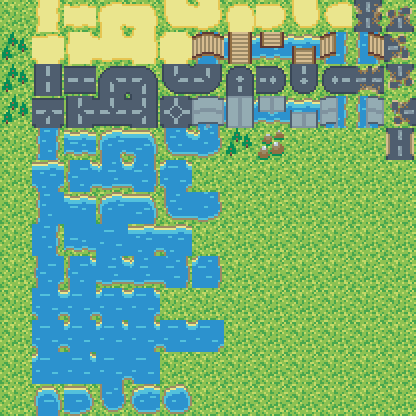
\includegraphics[scale = 1]{images/mapTileset.png}
    \caption{Sprite des tuiles}
    \label{fig:Advance Wars}
\end{figure}

\begin{figure}[h]
    \centering
    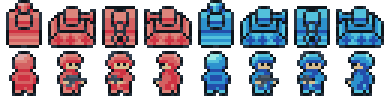
\includegraphics[scale = 1]{images/units.png}
    \caption{Sprite des unités}
    \label{fig:Advance Wars}
\end{figure}

\begin{figure}[h]
    \centering
    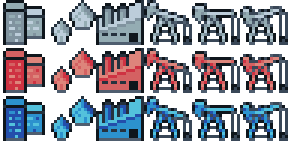
\includegraphics[scale = 1]{images/buildings.png}
    \caption{Sprite des bâtiments}
    \label{fig:Advance Wars}
\end{figure}
%\subsubsection{Les tuiles}

\newpage